I en underkategori inden for kunstig intelligens findes området maskinlæring. Maskinlæring spiller en stor rolle for selskaber, da maskinlæring anvendes til at behandle store mængder data, som maskinen her ud fra kan forudse fremtiden for firmaet. En fordel er at maskinlæring, ud fra de rette modeller, automatisk kan samle nyt data og holde sine forudsigelser opdateret. Maskinlæring gør det muligt for systemet at lære af sig selv ud fra data i stedet for, at det skal programmeres. 
\par
Ud fra maskinlæring bruges et stort udvalg af algoritmer og data som maskinen anvender når den skal trænes (altså lære af sig selv). Konceptet bruges for eksempel inden for e-handel, når maskinen lærer at promovere produkter på en hjemmeside. En model kunne være, at et system skal promovere produkter ud fra anmeldelser, kundens søgehistorik og måske anbefale produkter ud fra, hvad andre har købt sammen med et given produkt \cite{ML1}.
\par
Et andet område, som maskinlæring dagligt bruges indenfor, er eksempelvis Youtube, som er ejet af Google. En artikel udgivet af Google omhandler, hvordan maskinlæring anvendes til at anbefale seere nye videoer, baseret på deres adfærd. Google beskriver deres system som værende et af de største og mest sofistikerede systemer der eksisterer \cite{ML2}.
\par
Processen begynder med, at systemet udvælger en stor stikprøve på omkring en million videoer, baseret på nøgleord, søgning, videoers seertal og hvor seerne befinder sig. Fra denne mængde af videoer bliver der yderligere lavet en udvælgelse baseret på indholdet af videoen og seerenes præferencer. De højst rangerede videoer bliver derefter vist til brugeren. Målet er at udregne en seers forventede "watchtime", som er mængden af tid personen vil bruge på videoen. Dette system er et eksempel på et anvendelseområde af maskinlæring, hvor maskinen indsamler oplysninger om seereren, og trænes til at forudse, hvor lang tid seeren vil bruge på en given video \cite{ML2}.
\par
YouTube's maskinlæring er i form af \textit{deep learning} som beskrives senere i rapporten, og er baseret på Google's Google Brain som nu er blevet open-source ved navnet TensorFlow. Open-source betyder, at biblioteket eller frameworket er frit offentligt tilgængeligt med algoritmer, som alle kan anvende og modificere. Dette giver alle adgang til at kunne bruge maskinlæringsalgoritmer eller endda udvikle sine egne heraf, som er lovlige at udgive \cite{ML2}.
\par

\par
% Der er noget med YouTube i 1950'erne her
Det kan opsummeres, at der findes mange mulige måder at anvende maskinlæring på. Årsagen er den store vækst inden for teknologien som startede i 1950'erne, da man så potentialet i det. Denne teknologi er siden blevet anvendt til eksempelvis Youtube og e-handel. Disse mulige måder at anvende maskinlæringsalgoritmer på forekommer i biblioteker, som er gjort offentligt tilgængelige, og som vi derfor har mulighed at gøre brug af i vores projekt.


Maskinlæring er et stort og bredt område, så et mere konkret metodevalg vil før eller siden blive nødvendigt i dette projekt. Derfor vil analysen nu rette sig mod at finde overblik over konkrete maskinlæringsmetoder for at foretage en videre afgrænsning. 
% Introduktion til afsnittet
% Neural networking, Learning algorithms.
% Kun så specifikt som vi er i stand til inden problemløsningen
% Hvordan fungerer de og hvad bruges de til?

\subsubsection{Supervised learning} % Står det samme i næste sætning
\textit{Supervised learning} er en træningsmetode der bliver givet et datasæt, hvori de rigtige resultater er markerede, så træningsalgoritmen ved, hvordan den skal tilrette modellen der trænes. Dette kan sammenlignes med et menneske, som lærer ved at få feedback fra en underviser, som kender de rigtige svar \citep{Jeanmonod2018}.
\par
Et ofte brugt eksempel på et sæt af træningsdata er Iris-datasættet fra \cite{fisher1936}. Ved at bruge dette datasæt til at træne en læringsalgoritme, vil det blive i stand til at klassificere, hvilken af de tre arter i datasættet, som en irisblomst tilhører, ud fra mål af kron- og bægerblade.
\par
% Afsnit om support vektor machines
% Der findes forskellige metoder at bruge supervised learning på. En populær metode er en \textit{Support Vector Machine} (SVM), der bruges til regression og klassifikation. En SVM klassificerer data ved at lave en ikke-lineær separation i et multidimensionalt rum, der adskiller dataklasserne \cite{kotsiantis2007}. Antallet af dimensioner er det samme som antallet af egenskaber i dataet. Denne ikke-lineære adskillelse, laves ved lave en lineær adskillelse, i form af et hyperplan, i en højere dimension af rummet \cite{hastie01statisticallearning} [ILLUSTRATION]. En support vektor er et datapunkt der er placeret tæt på hyperplanet, og disse bruges til at maksimere margen mellem hyperplanet og dataklasserne.
% \\\\
% Forklarer at supervised learning har brug for træningsdata, hvilket ikke altid er godt.
Supervised learning metoder har brug for forudmarkeret data, for at kunne træne og give korrekte resultater. Størrelsen af et træningssæt vil ofte variere alt efter situationen, men der findes metoder til at bestemme den nødvendige mængde træningsdata i visse tilfælde \cite{Adcock1997}. Derfor præsenterer det en udfordring at bruge denne metode, hvis der ikke på forhånd er tilstrækkelig data tilgængelig. 
\par
% Lidt om feature selektion
Et andet aspekt der også er vigtigt at tage i betragtning, er \textit{feature selection}. Altså det at udvælge de egenskaber der er nødvendige at tage i betragtning for at få det korrekte eller bedste resultat. Én mulig tilgang til dette er at tage alle mulige egenskaber i betragtning for sig. I praksis kan dette imidlertid være vanskeligt at finde de nødvendige features uden tilstrækkeligt kendskab til det relevante fænomen. 
\par

% Afgrænsning
%I resten af projektet vil der ikke blive set nærmere på supervised learning da....
Supervised learning fravælges som metode i dette projekt, da der ikke er let tilgængelige datasæt med markeret data, der omhandler adfærd af sværme. Desuden er det uden for projektets rammer at sammensætte et tilstrækkeligt datasæt til dette formål. 

\subsubsection{Unsupervised learning}
% Lidt mere intro til unsupervised her.
\textit{Unsupervised learning} får, ligesom supervised learning, data som computeren kan arbejde med. Forskellen på disse to er, at unsupervised learning ikke får nogen mærkater på de data, der skal trænes på. Altså kan den ikke på samme måde trænes op, da den ikke kender resultaterne på eventuelle træningsdata. Der skal her laves analyser på data, og det kan derefter sorteres i undergrupper, hvilket kunne gøres ved hjælp at et beslutningstræ (eng. decision tree). 
\par
Et beslutningstræ er et godt eksempel på, hvordan unsupervised learning foregår, da programmet her skal finde nogle bestemte mønstre, som den skal gennemgå for alle data. 
\par 
Et eksempel på, hvordan det kunne se ud, kunne være som på figur \ref{Beslutningstrae}:
%%%%
\begin{figure}[H]
    \centering
    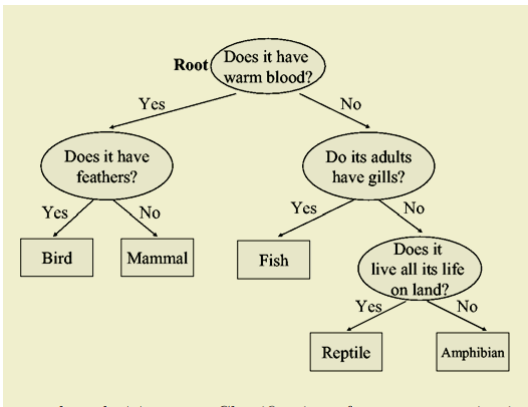
\includegraphics[width=0.7\textwidth]{figures/Beslutningstrae.png}
    \caption{Her ses et eksempel på et beslutningstræ som opdeler dyr, starter oppefra, og slutter i de firkantede kasser\cite{Bousquet2004}}
    \label{Beslutningstrae}
\end{figure}
%%%%
\par
% Sætning nummer 2 skal lige specificeres
Et eksempel på en måde at gøre dette på er ved hjælp af klyngeanalyser. Klyngeanalyser kan foregår på flere forskellige måder, der dog alle har mål relateret til enten gruppering eller segmentering af objekter til såkaldte \textit{clusters} [CITATION]. Sorteringen foregår således, at der via et brugerinput, bliver lavet et antal \textit{cluster centers}, og ud til disse bliver objekter sorteret således, at objekterne i samme klynge har mere til fælles med hinanden, end de har med objekter fra andre klynger.
\par
Et eksempel på en klyngeanalyse kunne være tre forskelligt farvede prikker, der skal deles op i tre klynger, som set på billedet nedenfor:
%%%%
 \begin{figure}[H]
    \centering
    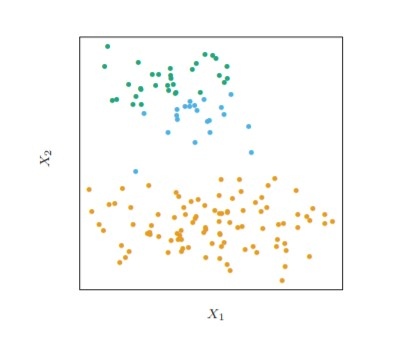
\includegraphics[width=0.7\textwidth]{figures/Cluster.jpg}
    \caption{Her ses et eksempel på en cluster analyse, hvor forskelligt farvede prikker deles op i 3 clusters \cite{Rodriguez-Perez1994}}
    \label{ClusterEksempel}
\end{figure}
%%%%
Disse prikker og farver kan repræsentere forskellig data, som programmet får eksternt. Dette kunne eksempelvis være data om tre forskellige dyr, som skulle deles op. Programmet vil her analysere de forskellige data, lede efter sammenhænge og mønstre og bruge disse til at dele dataet \cite{Rodriguez-Perez1994}. Denne opdeling sker ved hjælp af \textit{k-means algoritmen}. Denne algoritme tager de forskellige datapunkter i en matrix og laver et antal cluster centers \cite{K-Means}.
\par
% En anden vej at gå med unsupervised learning er \textit{association learning}, som eksempelvis kan bruges til markedsanalyse. Et eksempel på dette kunne være i en butik. Her vil der være variablerne $(X_1, X_2,...,X_n)$, som dækker over alle varer i butikken. Målet med en sådan analyse kan være at finde den samlede værdi af de variable som opstår flest gange. I dette eksempel er observationerne transaktioner, som eksempelvis dem der sker i en møbelforretning. Variablen $X_j$, hvor \textit{j} er hvilken vare der er tale om, vil få en binær værdi alt efter om varen er købt eller ej. Når alle varerene er kørt igennem algoritmen, er første observation færdig, og en ny observation kan gå i gang. De data der kommer ud af disse observationer, kan eksempelvis bruges til at lave et katalog til en butik, da de ved hjælp af dataene kan se hvilke varer der bliver solgt mest, hvilke kategorier der er mest populære, osv. \cite{Rodriguez-Perez1994}.

% Afgrænsning

\subsubsection{Reinforcement learning}
Ved denne type af læring, starter modellen typisk med en ren tavle \cite{deep-reinforcement-learning}. Modellen får ingen data med markerede svar, som i supervised learning, men skal i stedet prøve sig frem. En vigtig del af reinforcement learning, er at modellen får feedback på de handlinger den foretager. Dette sker igennem en fitness-funktion, som belønner modellen alt efter hvor tæt på målet den er. Dette kunne eksempelvis være hvor hurtigt modellen kan finde vej, fra ét punkt til et andet, eller hvor tæt den er på at gætte en tekststreng, eller hvor langt en simuleret bil har kørt [CITATION]. Fitness-funktionen beregner derefter en fitness-værdi, ud fra hvor godt modellen klarede sig, og ud fra denne feedback, kan modellen justere sig selv, og prøve igen, indtil den kommer i mål. Der findes utallige applikationer for denne type maskinlæring, dog skal der være et klart mål med modellen, noget programmøren gerne vil optimere, da modellen skal bruge en fitness-funktion for at kunne fungere.

% Policy based
% Value based
% Model based
Der findes tre forskellige tilgange til reinforcement learning med benævnelserne value based, policy based og model based. Value based handler om at optimere en værdifunktion som er en funktion som udregner den forventede gevinst. Maskinen vil derfor laver de handlinger som giver den største gevinst baseret på værdifunktionen. Hvis man tilføjer en "policy" funktion sammen med valuefunktionen, så er det en policy based reinforcement learning tilgang. Her forsøger maskinen at optimere både sin policyfunktion og sin valuefunktion. Policyfunktionen udregner hvilken handling maskinen skal tage. Under policyfunktioner findes der to typer heraf benævnt deterministic og stochastic. En deterministic funktion vil altid give den samme baseret på de samme inputs fra eksempelvis værdi funktionen. Derimod stochastic funktion har en sandsynlighed involveret som dækker resultere at der er sandsyndlighed i mellem de forskellige handlinger. Endeligt findes der en model baseret tilgang hvor der bliver lavet en model af miljøet som beskriver opførelsen for miljøet. \cite{RLapproaches}

\cite{deep-reinforcement-learning}. 
\par
% Lille eksempel på anvendelsen af reinforcement learning
% AlphaGo er ikke tidligere nævnt
% Ved ikke om det her eksempel skal med
Som tidligere nævnt, er AlphaGo et eksempel på \textit{reinforcement learning}. AlphaGo har undergået flere opgraderinger, og den nyeste version, AlphaGo Zero, har lært at spille Go uden menneskelig interaktion og uden at kende noget til spillet i forvejen \cite{alphago}. Den har spillet mod sig selv igen og igen, og hver gang fået feedback på, hvor godt den har klaret sig, som den så har brugt til at justere sit neurale netværk. På den måde bliver modellen bedre til at forudsige de næste træk den skal foretage, og på 40 dage blev AlphaGo Zero verdenmester i Go.
\par
En underkategori til reinforcement learning er Q-learning. Q learning er en værdi-baseret reinforcement learning, dette vil sige at der ligesom tidligere nævnt om reinforcement learning, er en fitness funktion som får point efter hvor godt den klare sig. Derudover starter Q-learning også med en ”ren  tavle”, altså ved den ikke noget om hvad det rigtige resultat er. Når der tales om Q learning, bruges det der hedder et Q-table, her udregnes den forventede værdi for et hvert skridt algoritmen kan tage, og den vil derefter tage den vej der forventes at give flest point\cite{Watkins1992}.
Et eksempel på hvordan Q learning fungerer, kunne være en simuleret agent der skal finde ud af en labyrint. Der vil være fire retninger at gå for hvert skridt den tager, og igennem et Q-table vil der udregnes hvilken retning der forventes at give flest point, altså være den hurtigste vej mod udgangen.  Her ville agenten starte på f.eks. 100 point, og få -1 for hvert skridt den tager. Målet vil således være at gennemføre labyrinten med så mange point som muligt, og jo flere point den får, jo højere en fitness værdi for den rute som den har taget, og algoritmen vil være mere tilbøjelig til at tage dele af dén rute igen\cite{ThomasSimonini2018}. 